\section{Exécution \& tests} % (fold)
\label{sec:execution}

Pour ce projet, nous avons effectué des tests de validation sur les fonctions algébriques, afin de s'assurer que celles-ci marchaient correctement, et pouvoir plus facilement isoler les problèmes. 
De même, le code a été segmenté pour permettre une lecture plus aisée de l'ordre dans lequel s'effectuent les diverses opérations.

\section{Performances} % (fold)
\label{sec:perf}

Une série de tests est lancée sur différentes tailles de matrice plusieurs fois, afin d'obtenir des temps d'exécution moyens. Nous avons remarqué que pour des matrices de taille croissantes, des erreurs de calcul apparaissaient. Ainsi, pour des matrics de taille $30 \times 30$, les erreurs commençaient à être significatives dans le calcul du dtrsm (de l'ordre de $0.1$).\\
Les courbes de performances ont été tracées avec gnuplot et permettent de savoir où le programme passe le plus de temps (Fig. \ref{fig:diff}). On peut voir que pour des dimensions de matrice de plus en plus grandes, c'est surtout le calcul de la multiplication qui augmente. En effet, nous ne faisons pas varier le nombre de processus; la charge de chaque processus augmente donc fortement.

\begin{figure}[H]
\centering
% \includegraphics[width=0.8\textwidth]{diff.png}
\caption{Temps d'exécution des différentes parties du programme}
\label{fig:diff}
\end{figure}

Comme l'indique la courbe de la Fig. \ref{fig:sp}, la parallélisation s'améliore avec la taille du problème. Nous avons fait les comparaisons avec MKL, et nous pouvons voir que nous sommes plus rapides pour des matrices de dimensions supérieures à $1000\times1000$, obtenant toutefois des performances moindres pour des tailles inférieures. Il faut cependant tenir compte du fait que MKL est déjà optimisé, et nos communications ralentissent donc (trop) le programme.

\begin{figure}[H]
\centering
% 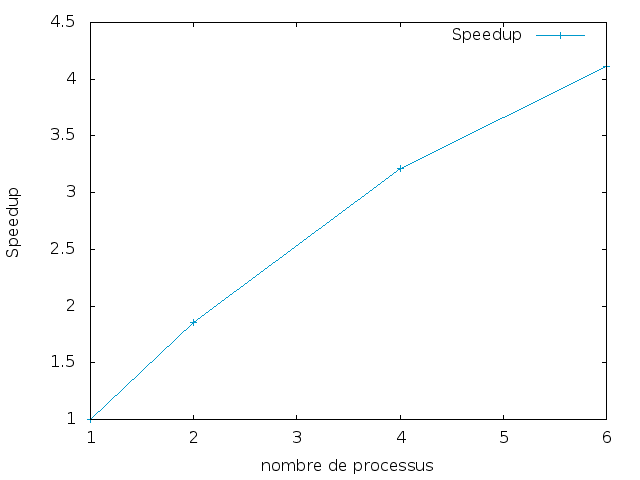
\includegraphics[width=0.8\textwidth]{Speedup.png}
\caption{Accélération de notre programme par rapport au code séquentiel}
\label{fig:sp}
\end{figure}

% section \ (end)
